%%
%% Author: Moritz
%% 18.03.2018
%%

% Preamble
\documentclass[../../Pflichtenheft.tex]{subfiles}
\begin{document}
    \subsection{Reservierung}
        \begin{figure}[ht!]
            \begin{center}
                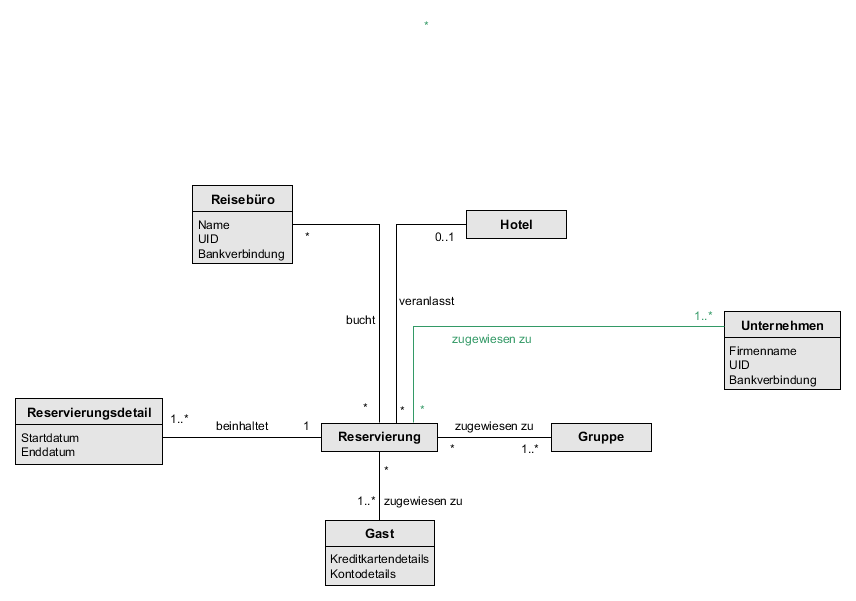
\includegraphics[width=0.7\linewidth]{assets/reservierung.png}
                \caption{Objekt 'Reservierung'} \label{reservierung_model}
            \end{center}
        \end{figure}Das Objekt 'Reservierung' dient als Container für Reservierungsdetails. Zudem
    ist die Reservierung mit dem Auftraggeber der Reservierung verknüpft. Das kann
    ein Unternehmen, ein Individualgast oder eine Reisegruppe sein. Die Reservierungen
    werden hierbei vom Hotel oder sogar direkt vom Reisebüro vorgenommen. Die Reservierungsdetails
    dienen dazu für eine Reservierung mehrere Zimmer zu reservieren mit den entsprechenden Zusatzinformationen.
    (siehe Detailklasse 'Reservierungsdetails')
\end{document}